%\section{Outline}
%\input{includes/thesis}
%Given a $m \times n$ system of equations: 
%\section*{Define arithmetic operations ($+, -, \times$) on matrices}
% \section*{Introduction}


%\subsubsection*{Objectives}
%\begin{itemize}
%	\item Calculate length of a vector
%	\item Calculate dot products
%	\item Use dot product to determine  
%\end{itemize}


\subsubsection*{Announcements}
\begin{outline}
\1[-] Homework due
\1[-] Exam Next X
\end{outline} 


\subsubsection*{Learning outcomes}
Be able to:
\begin{itemize}
	% \item Identify a $m \times n$ matrix
	\item Represent a linear system of equations as a ($m \times n$) matrix equation
	\item Write a linear combination in matrix form 
	\item Solve a matrix-vector equation
	\item View a matrix equation as finding linear combo. of columns of $A$ to produce vector ${\bf b}$
	% \item Find a difference matrix
	\item Introduce inverse of matrix
\end{itemize}






\rule[0.01in]{\textwidth}{0.0025in}
% ---------------------------------------------------- % 


%
%%
%%%						  
%%%% SECTION:  Matrices
%%%
%%
%
\section{Matrices}

% DEFINITION: Matrix Notation
 \begin{tcolorbox}[colback=yellow!10!,colframe=gray!15!]
 \begin{definition}[Matrix]
A  \textbf{matrix}, denoted with capital letters (e.g,. $A, B, C, X$), is an $m \times n$ rectangular array of numbers.   In general $a_{ij}$ is used to denote the $i$-th row and $j$-th column, (i.e.,  $(i,j)$-th entry).  Thus, if $A$ is an $m \times n$ matrix, then

\[ 
A =  \begin{bmatrix} 
	a_{11} & a_{12} & a_{13}	& \cdots & a_{1n} \\
 	a_{21} & a_{22} & a_{13}	& \cdots & a_{2n} \\
  	a_{31} & a_{32} & a_{33}	& \cdots & a_{3n} \\
	\vdots 	&	&	& \cdots & \vdots \\
    	a_{m1} & a_{m2} & a_{m3}	& \cdots & a_{mn} \\
    \end{bmatrix}  = (a_{ij})
 \]
 \end{definition}	 
 \end{tcolorbox} 








% EXAMPLE
\begin{example}
A $3 \times 4$ matrix is given below: 
\[ A = \begin{bmatrix}  1& 2& 3 & 4\\ 5 & 6 & 7  & 8\\ 9 & 10 & 11 & 12 \end{bmatrix} \]
\end{example}

\rule[0.01in]{\textwidth}{0.0025in}
% ---------------------------------------------------- % 



\subsection*{Matrix-vector Product}
The matrix-vector product, $A{\bf x}$, can be viewed as a linear combination\footnote{Linar combinations are \textbf{the} key to linear algebra.} of the columns of $A$.  In particular, let 
\[  {\bf u} = \begin{bmatrix}  1 \\-1 \\0 \end{bmatrix}, {\bf v} = \begin{bmatrix} 0 \\ 1 \\ -1 \end{bmatrix}, {\bf w} = \begin{bmatrix} 0 \\ 0 \\ 1  \end{bmatrix}
\]
and ${\bf x}=\begin{bmatrix}  x_1 \\x_2 \\x_3 \end{bmatrix}$, then the linear combination

\[  x_1 {\bf u} + x_2 {\bf v} + x_3 {\bf w} = x_1 \begin{bmatrix}  1 \\-1 \\0 \end{bmatrix} + x_2\begin{bmatrix} 0 \\ 1 \\ -1 \end{bmatrix} + x_3 \begin{bmatrix} 0 \\ 0 \\ 1  \end{bmatrix} = \begin{bmatrix} x_1 \\ x_2 - x_1 \\ x_3 - x_2   \end{bmatrix}
\]

{\bf *}Then $ \begin{bmatrix} x_1 \\ x_2 - x_1 \\ x_3 - x_2   \end{bmatrix}$ can be written as, 
\[ A{\bf x}  = \begin{bmatrix}  1 & 0 & 0 \\-1 & 1 & 0 \\0 & -1 & 1 \end{bmatrix}  \begin{bmatrix}  x_1 \\x_2 \\x_3 \end{bmatrix} \]

where the vectors ${\bf u}, {\bf v}$, and ${\bf w}$ are the columns of $A$.

The matrix $A$ times the vector ${\bf x}$ is the same as the combination of the columns of $A$.  

\rule[0.01in]{\textwidth}{0.0025in}
% ---------------------------------------------------- % 


\textbf{Alternatively}, $A{\bf x}$ can be viewed as dot products of the rows of $A$ with the vector ${\bf x}$.  In particular, 
\[  A {\bf x} = \begin{bmatrix}  1 & 0 & 0 \\-1 & 1 & 0 \\0 & -1 & 1 \end{bmatrix}  \begin{bmatrix}  x_1 \\x_2 \\x_3 \end{bmatrix} 
=   \begin{bmatrix}  (1, 0, 0) \cdot (x_1,x_2,x_3) \\ (-1, 1, 0) \cdot (x_1,x_2,x_3) \\ (0, -1, 1) \cdot (x_1,x_2,x_3) \end{bmatrix}
 \]
 
 \textbf{Computationally}, the elements of the resulting vector in a matrix-vector product are given by:
 

\begin{align*}
	b_{i} &= \sum_{k=1}^n  a_{ik} x_{k}  \hspace{0.5cm}  \forall i \in \{1, 2, \dots m \}
\end{align*}



% ---------------------------------------------------- % 
\rule[0.01in]{\textwidth}{0.0025in}
% ---------------------------------------------------- % 

 
 
 
 
 
 
 
 
 
 
%
%%
%%%						  
%%%% SECTION:  Linear Equations 
%%%
%%
%
\section{Linear Equations}

There are \textbf{two} (symmetric, or inverse) problems associated with the equation $A{\bf x} = {\bf b}$:
\begin{enumerate}
	\item Find {\bf b} given {\bf x}
	\item {\color{blue}Find} {\bf x} given  {\bf b}
\end{enumerate}

The analog of the second problem is familiar, \textbf{solve} $ax = b$, for example, solve $2x = 5$.  

With a system of equations, if $A$ is invertible, from  ${\bf b}$ we can recover ${\bf x}$.  
\[  A{\bf x} = {\bf b}  \;\;\;  \Longleftrightarrow   \;\;\;  {\bf x} = A^{-1} {\bf b} \] 


In our working example,
\[  A {\bf x} =  \begin{bmatrix} x_1 \\ x_2 - x_1 \\ x_3 - x_2   \end{bmatrix} = {\bf b} \]

In other words, ${\bf b}$, were differences  of the $x_i$'s
\[   \begin{bmatrix} b_1 \\ b_2  \\ b_3   \end{bmatrix}  =  \begin{bmatrix} x_1 - 0 \\ x_2 - x_1 \\ x_3 - x_2   \end{bmatrix}  \]

and ${\bf x}$ will be the sum of the $b_i$'s!

\[   \begin{bmatrix} x_1 \\ x_2  \\ x_3   \end{bmatrix}  =  \begin{bmatrix} b_1 + 0  \\ b_1 + b_2 \\ b_2 + b_3   \end{bmatrix}  \]

This is no accident or coincidence.  

% ---------------------------------------------------- % 
\rule[0.01in]{\textwidth}{0.0025in}
% ---------------------------------------------------- % 

 
 
 
 
 \subsection{Dependent}
If the columns of $A$ are dependent, then $A {\bf x} = {\bf 0}$ has infinite solutions.  

% If the columns of $A$ are independent, then $A {\bf x} = {\bf 0}$ has one solution, namely ${\bf x} = {\bf 0}$.  $A$ is invertible.  However, if the columns of $A$ are dependent, then $A {\bf x} = {\bf 0}$ has infinite solutions.  


 
 
 
 

% EXAMPLE
\begin{example}
If $ A = \begin{bmatrix}  1& 2\\ 1 & 2  \end{bmatrix} $, then $A {\bf x} = {\bf 0}$ has many solutions.  For instance, three solutions are:  $(-2, 1), (-4, 2), \text{ and } (2, -1)$
\end{example}

\rule[0.01in]{\textwidth}{0.0025in}
% ---------------------------------------------------- % 



\subsection{Applied Problems}

\begin{questions}
	\question $ \begin{array}{rcl}& & \\ x_1 - 3x_2 & = & 2 \\ 2 x_2 & = & 6 \end{array}$


\question  $ \begin{array}{rcl}& & \\& &  \\ x_1 + x_2 +x_3 & = & 8 \\ 2 x_2 +x_3 & = & 5 \\ 3x_3 & = & 9 \end{array}$ \\

 % -----------  C ---------------
\question  $ \begin{array}{rcl}
& & \\ 
& & \\ 
x_1 +2x_2 + 2x_3 + x_4 & = & 5  \\
          3x_2 +  x_3 + -2x_4 & = & 1 \\ 
                         -x_3 + 2x_4 & = & -1 \\ 
                                      4x_4 & = & 4   \end{array}$

\question  $ \begin{array}{rcl}
& & \\ 
& & \\ 
& & \\ 
& & \\ 
x_1 +x_2 + x_3 + x_4  + x_5 & = & 5  \\
          2x_2 +  x_3 + -2x_4 + x_5 & = & 1 \\ 
                         4x_3 + x_4-2 x_5 & = & 1 \\ 
                                      x_4 -3 x_5 & = & 0 \\
                                                    2x_5 & = & 2   \end{array}$



 
 


% - Problem 2
 
\question $\begin{array}{rcl} x_1 + x_2 +x_3 & = & 8 \\ 2 x_2 +x_3 & = & 5 \\ 3x_3 & = & 9 \end{array}$
 
 
 
 \question  In the process of photosynthesis, plants use radiant energy from sunlight to convert carbon dioxide ($CO_2$) and water ($H_2O$) into glucose ($C_6H_{12}O_6$) and oxygen ($O_2$).  The chemical equation of the reaction is of the form

\[ x_1 CO_2 + x_2 H_2O \longrightarrow x_3 O_2 + x_4 C_6H_{12}O_6 \]

To balance the equation, we must choose $x_1$, $x_2$, $x_3$, and $x_4$ so that the numbers of carbon, hydrogen, and oxygen atoms are the same on each side of the equation.   Model the problem using a system of linear equations, then represent it in matrix form.  




\question A fruit grower raises two crops, apples and oranges.  Each of these crops is shipped to three different outlets, see Table below.  The profit per unit for apples is \$3.50 and the profit per orange is \$6.00.  Find the profit from each outlet.




\begin{tabular}{c|ccc}
  & \multicolumn{3}{c}{Quantity sent to Outlets }  \\ 
 \hline
 Apples &   125  &  100  & 75 \\ 
  Oranges &   100  &  175  & 125 \\ 
 
 \end{tabular}






\question Find a polynomial that relates the periods of the first three planets to their mean distances from the sun, as shown in Table below.  Then test the accuracy of the fit by using the polynomial to calculate the period of Mars.  (Distance is measured in astronomical units, and period is measured in years.  Source: CRC Handbook of Chemistry and Physics).

\begin{tabular}{l|cccccc}
 \hline
 Planet & Mercury & Venus  & Earth  &  Mars  &  Jupiter  & Saturn\\
 \hline
Mean Distance & 0.387 & 0.723  & 1.0  &  1.523  &  5.203  & 9.541\\
Period & 0.241 & 0.615  & 1.0  &  1.881  &  11.861  & 29.457\\
 \hline 
\end{tabular}







\question   Suppose a city consists of sets of one-way streets.  The average hourly volume of traffic entering and leaving each intersection is given by the diagram.  Determine the amount of traffic between each intersection (See Figure below).
        \begin{figure}[htbp] %  figure placement: here, top, bottom, or page
           \centering
           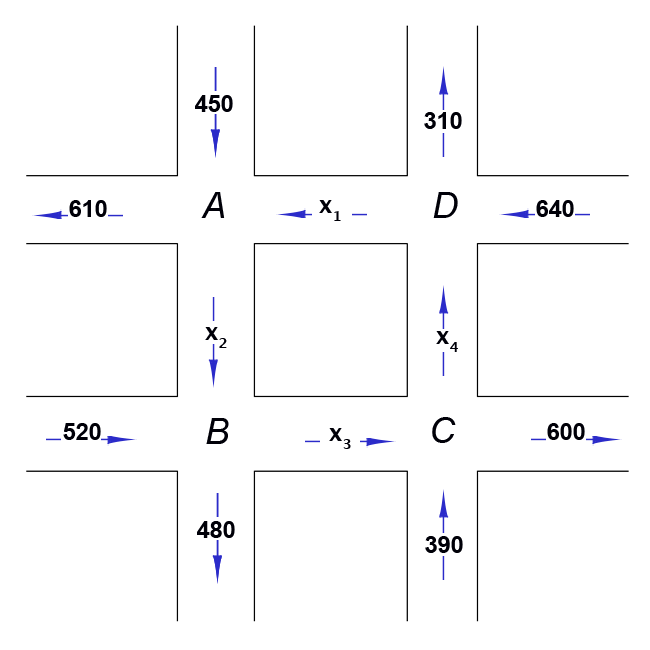
\includegraphics[width=4in]{figures/trafficflow.png} 
           \caption{Average Hourly Volume of Traffic in City Center}
           \label{fig:trafficflow}
        \end{figure}
        
   		


\end{questions}




\rule[0.01in]{\textwidth}{0.0025in}
% ---------------------------------------------------- % 


\subsubsection*{Next time...}
Section 2.1: Vectors and Linear Equations





\subsubsection*{Problems from the Book}
\textsection1.3: \#2, 3, 4, 8, 10









%\begin{tcolorbox}[colback=yellow!10!,colframe=gray!15!]
%\begin{theorem}[Cauchy-Schwarz Inequality]
%If ${\bf x} $ and ${\bf y} $ are vectors (in an inner product space) then
 %\[ |  {\bf x} \cdot {\bf y} | \le ||{\bf x}|| \,  ||{\bf y}|| \]
 %\end{theorem}	 
%\end{tcolorbox} 



